\documentclass[a4paper]{article}
\usepackage[utf8]{inputenc}
\usepackage[russian,english]{babel}
\usepackage[T2A]{fontenc}
\usepackage[left=10mm, top=20mm, right=18mm, bottom=15mm, footskip=10mm]{geometry}
\usepackage{indentfirst}
\usepackage{amsmath,amssymb}
\usepackage[italicdiff]{physics}
\usepackage{graphicx}
\usepackage{caption}
\usepackage{float}
\renewcommand{\thefootnote}{\fnsymbol{footnote}}
\usepackage{tablefootnote}
\usepackage{footmisc}
\usepackage[parfill]{parskip}
\usepackage[utf8]{inputenc}\newcommand{\approxtext}[1]{\ensuremath{\stackrel{\text{#1}}{\approx}}}
\graphicspath{{images/}}
\DeclareGraphicsExtensions{.pdf,.png,.jpg}
\usepackage{wrapfig}
\captionsetup{labelformat=empty}
\usepackage{caption}
\captionsetup[figure]{name=Рисунок}
\captionsetup[table]{name=Таблица}
  
\title{\textbf{Отчет о выполненой лабораторной работе 2.1.2}}
\date{}
\author{Котляров Михаил, Б01-402}

\begin{document}

\maketitle
	
	\section{Введение}
	
	\textbf{Цель работы:} : определить отношение $\gamma = \frac{C_p}{C_v}$ для воздуха и углекислого газа по измерению давления в стеклянном сосуде.

	\textbf{Оборудование:} стеклянный сосуд; U-образный жидкостный манометр (жидкость - вода); резиновая груша; газгольдер с углекислым газом; психрометр.
	
	\section{Экспериментальная установка и некоторые теоретические сведения}

	Используемая для опытов экспериментальная установка состоит из стеклянного сосуда А, снабженного краном К, и U-образного жидкостного манометра, измеряющего избыточное давление газа в сосуде. Схема установки показана на Рис. 1.\\
\begin{figure}[h!]
\centering{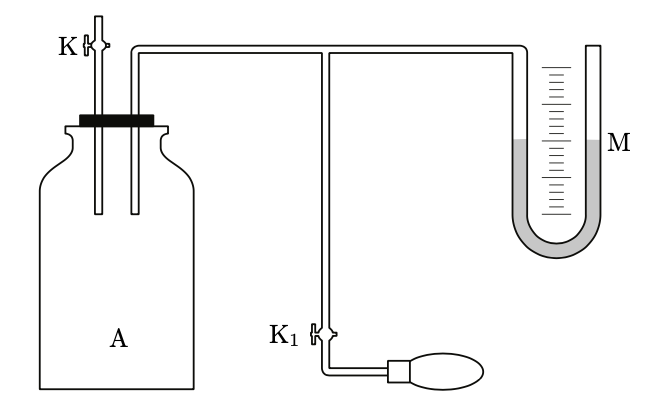
\includegraphics[width=1\textwidth]{ustanovka.jpg}}
\caption[]{\label{} Рис. 1. Экспериментальная установка}
\end{figure}
	Избыточное давление создаётся с помощью резиновой груши, соединённой с сосудом трубкой с краном $K_1$.
	В начале опыта  в стеклянном сосуде А находится исследуемый газ при комнатной температуре $T_1$ и давлении $P_1$, несколько превышающем атмосферное давление  $P_0$. После открытия крана К, соединяющего сосуд А с атмосферой, давление и температура газа будут понижаться. Это уменьшение температуры приближённо можно считать адиабатическим, поскольку $\Delta t_P \ll \Delta t_T$, $\Delta t_P$ и $\Delta t_T$ обозначают соответственно выравнивание давления и температуры.\\
	Обозначим состояние газа после повышения давления в сосуде и выравнивания температуры с комнатной индексом 1, сразу после открытия крана $K$ индексом 2, после закрытия крана $K$ и изохорного нагревания индексом 3. Из уравнений адиабаты и Клапейрона получим
\begin{equation*}
	(\frac{P_1}{P_2})^{\gamma-1} = (\frac{T_1}{T_2})^{\gamma}.
\end{equation*}
По закону Гей-Люссака для изохорного процесса
\begin{equation*}
	\frac{P_2}{T_2} = \frac{P_3}{T_3} = \frac{P_3}{T_1}.
\end{equation*}
С учетом того, что $P_1 = P_0 + \rho g h_1$, $P_2 = P_0$, $P_3 = P_0 + \rho g h_2$,
\begin{equation*}
	\gamma = \frac{\ln(P_1/P_0 )}{\ln(P_1/P_3)},
\end{equation*}
\begin{equation*}
	\gamma = \frac{\ln(1 + \rho g h_1/P_0 )}{\ln(1 + \rho g h_1/P_0) - {\ln(1 + \rho g h_2/P_0)}} \approx \frac{h_1}{h_1 - h_2}.
	\eqno(1)
\end{equation*}


\section{Выполнение}

\subsection{Воздух}
\begin{enumerate}


\item Перед началом измерений оценим время установления равновесия.  Для этого закроем кран $K$ и увеличим с помощью груши давление на 21,9 см.вод.ст.. Давление установилось примерно через 40 секунд, поэтому в дальнейших измерениях время установления равновесия бралось 40-50 с.

\item Проведем теперь 3 серии измерения. Для каждого времени открытия $\Delta t$ будем нагнетать давление в сосуде, ждать пока давление перестанет меняться, фиксировать $\Delta h_1$. Затем откроем кран $K$ на время $\Delta t$, подождем, пока система придет в равновесие. Зафиксируем $\Delta h_2$. Эти действия проделаем 5-6 раз для трех диапазонов $\Delta t$.
\item Полученные данные приведены в следующих таблицах
\begin{table}[h!]
    \centering
    \begin{tabular}{|c|c|c|c|c|}
        \hline
        $h_1, \text{см}$ & $h_2, \text{см}$ & $\gamma$ & $\sigma_\gamma^{\text{сист}}$ & $\varepsilon_\gamma^{\text{сист}}, \%$ \\
        \hline
        $14.9 \pm 0.2$ & $2.5 \pm 0.2$ & $1.202$ & $0.020$ & $1.64$ \\ \hline
        $10.1 \pm 0.2$ & $1.9 \pm 0.2$ & $1.232$ & $0.031$ & $2.48$ \\ \hline
        $8.3 \pm 0.2$ & $2.0 \pm 0.2$ & $1.317$ & $0.043$ & $3.27$ \\ \hline
        $7.8 \pm 0.2$ & $1.6 \pm 0.2$ & $1.258$ & $0.041$ & $3.29$ \\ \hline
        $7.9 \pm 0.2$ & $1.9 \pm 0.2$ & $1.317$ & $0.045$ & $3.43$ \\ \hline
    \end{tabular}
    \caption{Таблица 1. $\Delta t \approx 0,5 c$}
\end{table}

\begin{table}[h!]
    \centering
    \begin{tabular}{|c|c|c|c|c|}
        \hline
        $h_1, \text{см}$ & $h_2, \text{см}$ & $\gamma$ & $\sigma_\gamma^{\text{сист}}$ & $\varepsilon_\gamma^{\text{сист}}, \%$ \\
        \hline
        $19.1 \pm 0.2$ & $4.8 \pm 0.2$ & $1.336$ & $0.019$ & $1.44$ \\ \hline
        $18.7 \pm 0.2$ & $4.8 \pm 0.2$ & $1.345$ & $0.020$ & $1.49$ \\ \hline
        $18.5 \pm 0.2$ & $4.6 \pm 0.2$ & $1.331$ & $0.020$ & $1.48$ \\ \hline
        $19.3 \pm 0.2$ & $4.8 \pm 0.2$ & $1.331$ & $0.019$ & $1.42$ \\ \hline
        $19.4 \pm 0.2$ & $4.5 \pm 0.2$ & $1.302$ & $0.018$ & $1.38$ \\ \hline
        $19.1 \pm 0.2$ & $4.6 \pm 0.2$ & $1.317$ & $0.019$ & $1.42$ \\ \hline
    \end{tabular}
    \caption{Таблица 2. $\Delta t \approx 0,5-1,5c$}
\end{table}

\begin{table}[h!]
    \centering
    \begin{tabular}{|c|c|c|c|c|}
        \hline
        $h_1, \text{см}$ & $h_2, \text{см}$ & $\gamma$ & $\sigma_\gamma^{\text{сист}}$ & $\varepsilon_\gamma^{\text{сист}}, \%$ \\
        \hline
        $20.2 \pm 0.2$ & $4.3 \pm 0.2$ & $1.270$ & $0.016$ & $1.29$ \\ \hline
        $19.0 \pm 0.2$ & $4.2 \pm 0.2$ & $1.284$ & $0.018$ & $1.38$ \\ \hline
        $18.9 \pm 0.2$ & $4.2 \pm 0.2$ & $1.286$ & $0.018$ & $1.39$ \\ \hline
        $19.5 \pm 0.2$ & $4.3 \pm 0.2$ & $1.283$ & $0.017$ & $1.35$ \\ \hline
        $19.5 \pm 0.2$ & $4.2 \pm 0.2$ & $1.275$ & $0.017$ & $1.34$ \\ \hline
    \end{tabular}
    \caption{Таблица 3. $\Delta t \approx 5 c$}
\end{table}

\item Индексами 1, 2, 3 обозначены значения для соответствующих серий измерений. Средние значения показателей равны $\bar{\gamma}_1 = 1,265$, $\bar{\gamma}_2 = 1,327$, $\bar{\gamma}_3 = 1,279$. Погрешности:
\begin{equation*}
	\sigma_\gamma^{\text{случ}} = \sqrt{\frac{\sum_{i=1}^{n}(\bar{\gamma} - \gamma_i)^2}{n(n-1)}}
\end{equation*}
\begin{align}
    \sigma_{\gamma_1}^{\text{случ}} &= 0,005 & \sigma_{\gamma_2}^{\text{случ}} &= 0,0003 & \sigma_{\gamma_3}^{\text{случ}} &= 0,0003
\end{align}
\begin{equation*}
	\sigma_\gamma^{\text{сист}} = max(\sigma_\gamma^{\text{сист}}) = 0,0451
\end{equation*}
Поэтому случайными погрешностями в 2 и 3 сериях можно принебречь.
\begin{equation*}
	\sigma_\gamma = \sqrt{{\sigma_\gamma^{\text{сист}}}^2 + {\sigma_\gamma^{\text{случ}}}^2}
\end{equation*}
\begin{align}
    \sigma_{\gamma_1} &= 0,0454 & \sigma_{\gamma_2} &= 0,0451 & \sigma_{\gamma_3} &= 0,0451
\end{align}

\item Построим по МНК график зависимости показателя адиабаты для воздуха от времени открытия крана $\gamma(\Delta t)$.
\begin{figure}[h!]
\centering{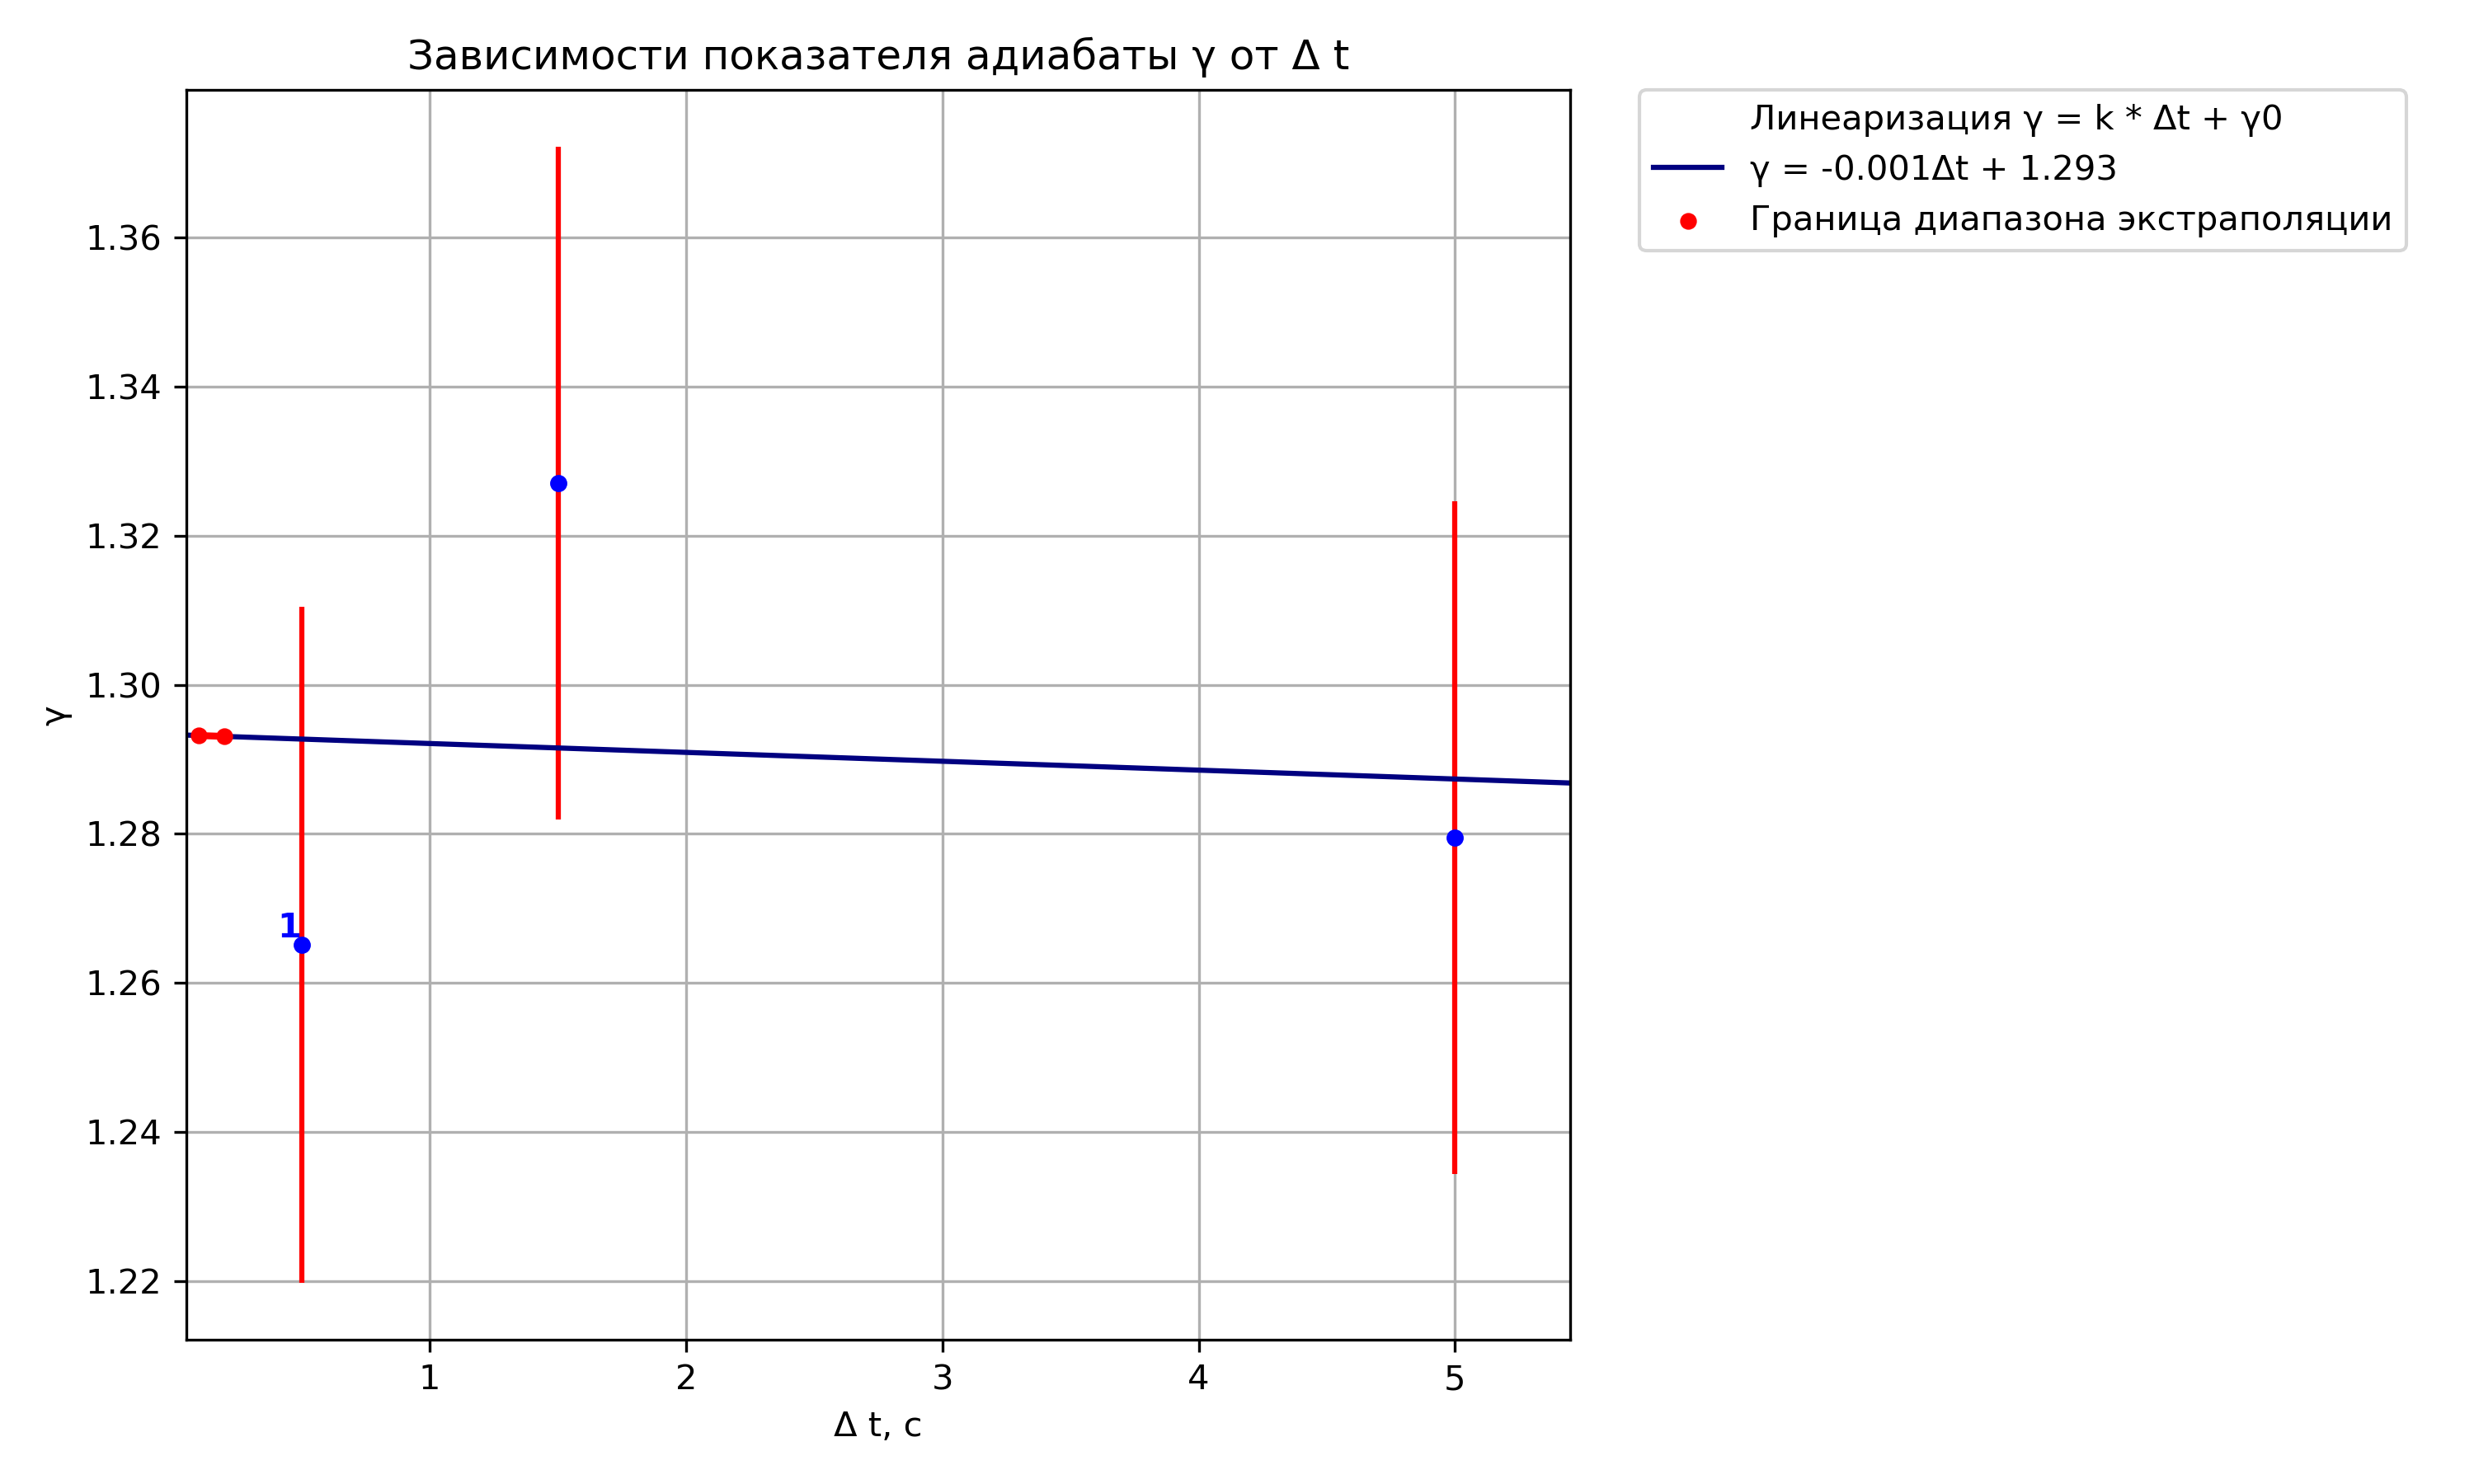
\includegraphics[width=1\textwidth]{graph1.png}}
\caption[]{\label{} График №1 Зависимость показателя адиабаты для воздуха от времени открытия крана $\gamma(\Delta t)$}
\end{figure}
\begin{equation*}
	k = -0,001 \pm 0,008
\end{equation*}
\begin{equation*}
	\gamma_0 = 1,293 \pm 0,015
\end{equation*}
По полученным параметрам прямой вычисли диапазон показателя адиабаты при $\Delta t$ = 0,1-0,2с.
\begin{equation*}
	\gamma_{\text{воз}} = 1,293
\end{equation*}
\begin{equation*}
	\sigma_{\gamma_{\text{воз}}} = \sqrt{(\Delta t\sigma_k)^2 + \sigma_{\gamma_0}^2} = \sqrt{0,0008^2 + 0,015^2} = 0,015
\end{equation*}
\begin{equation*}
	\gamma_{\text{воз}} = 1,293 \pm 0,015
\end{equation*}
\end{enumerate}


\subsection{Углекислый газ}

Проделаем все то же самое для углекислого газа
\clearpage
\begin{table}[h!]
    \centering
    \begin{tabular}{|c|c|c|c|c|}
        \hline
        $h_1, \text{см}$ & $h_2, \text{см}$ & $\gamma$ & $\sigma_\gamma^{\text{сист}}$ & $\varepsilon_\gamma^{\text{сист}}, \%$ \\
        \hline
        $9.0 \pm 0.2$ & $1.7 \pm 0.2$ & $1.233$ & $0.034$ & $2.79$ \\ \hline
        $8.9 \pm 0.2$ & $1.9 \pm 0.2$ & $1.271$ & $0.037$ & $2.92$ \\ \hline
        $9.1 \pm 0.2$ & $2.0 \pm 0.2$ & $1.282$ & $0.037$ & $2.88$ \\ \hline
        $8.9 \pm 0.2$ & $1.9 \pm 0.2$ & $1.271$ & $0.037$ & $2.92$ \\ \hline
        $8.9 \pm 0.2$ & $1.9 \pm 0.2$ & $1.271$ & $0.037$ & $2.92$ \\ \hline
    \end{tabular}
    \caption{Таблица 4. $\Delta t \approx 0,5 c$}
\end{table}

\begin{table}[h!]
    \centering
    \begin{tabular}{|c|c|c|c|c|}
        \hline
        $h_1, \text{см}$ & $h_2, \text{см}$ & $\gamma$ & $\sigma_\gamma^{\text{сист}}$ & $\varepsilon_\gamma^{\text{сист}}, \%$ \\
        \hline
        $8.9 \pm 0.2$ & $1.9 \pm 0.2$ & $1.271$ & $0.037$ & $2.92$ \\ \hline
        $8.9 \pm 0.2$ & $1.7 \pm 0.2$ & $1.236$ & $0.035$ & $2.83$ \\ \hline
        $9.1 \pm 0.2$ & $1.9 \pm 0.2$ & $1.264$ & $0.036$ & $2.84$ \\ \hline
        $9.1 \pm 0.2$ & $1.6 \pm 0.2$ & $1.213$ & $0.033$ & $2.71$ \\ \hline
        $8.9 \pm 0.2$ & $1.9 \pm 0.2$ & $1.271$ & $0.037$ & $2.92$ \\ \hline
    \end{tabular}
    \caption{Таблица 5. $\Delta t \approx 0,5-1,5c$}
\end{table}

\begin{table}[h!]
    \centering
    \begin{tabular}{|c|c|c|c|c|}
        \hline
        $h_1, \text{см}$ & $h_2, \text{см}$ & $\gamma$ & $\sigma_\gamma^{\text{сист}}$ & $\varepsilon_\gamma^{\text{сист}}, \%$ \\
        \hline
        $8.9 \pm 0.2$ & $1.5 \pm 0.2$ & $1.203$ & $0.033$ & $2.74$ \\ \hline
        $8.7 \pm 0.2$ & $1.5 \pm 0.2$ & $1.208$ & $0.034$ & $2.82$ \\ \hline
        $9.1 \pm 0.2$ & $1.6 \pm 0.2$ & $1.213$ & $0.033$ & $2.71$ \\ \hline
        $9.0 \pm 0.2$ & $1.5 \pm 0.2$ & $1.200$ & $0.032$ & $2.70$ \\ \hline
        $9.1 \pm 0.2$ & $1.5 \pm 0.2$ & $1.197$ & $0.032$ & $2.67$ \\ \hline
    \end{tabular}
    \caption{Таблица 6. $\Delta t \approx 5 c$}
\end{table}

\begin{align}
    \sigma_{\gamma_1}^{\text{случ}} &= 0,0005 & \sigma_{\gamma_2}^{\text{случ}} &= 0,0008 & \sigma_{\gamma_3}^{\text{случ}} &= 0,0004
\end{align}
\begin{equation*}
	\sigma_\gamma^{\text{сист}} = max(\sigma_\gamma^{\text{сист}}) = 0,037
\end{equation*}
\begin{align}
    \sigma_{\gamma_1} &= 0,037 & \sigma_{\gamma_2} &= 0,037 & \sigma_{\gamma_3} &= 0,037
\end{align}

Построим по МНК график зависимости показателя адиабаты для углекислого газа от времени открытия крана $\gamma(\Delta t)$.
\clearpage
\begin{figure}[h!]
\centering{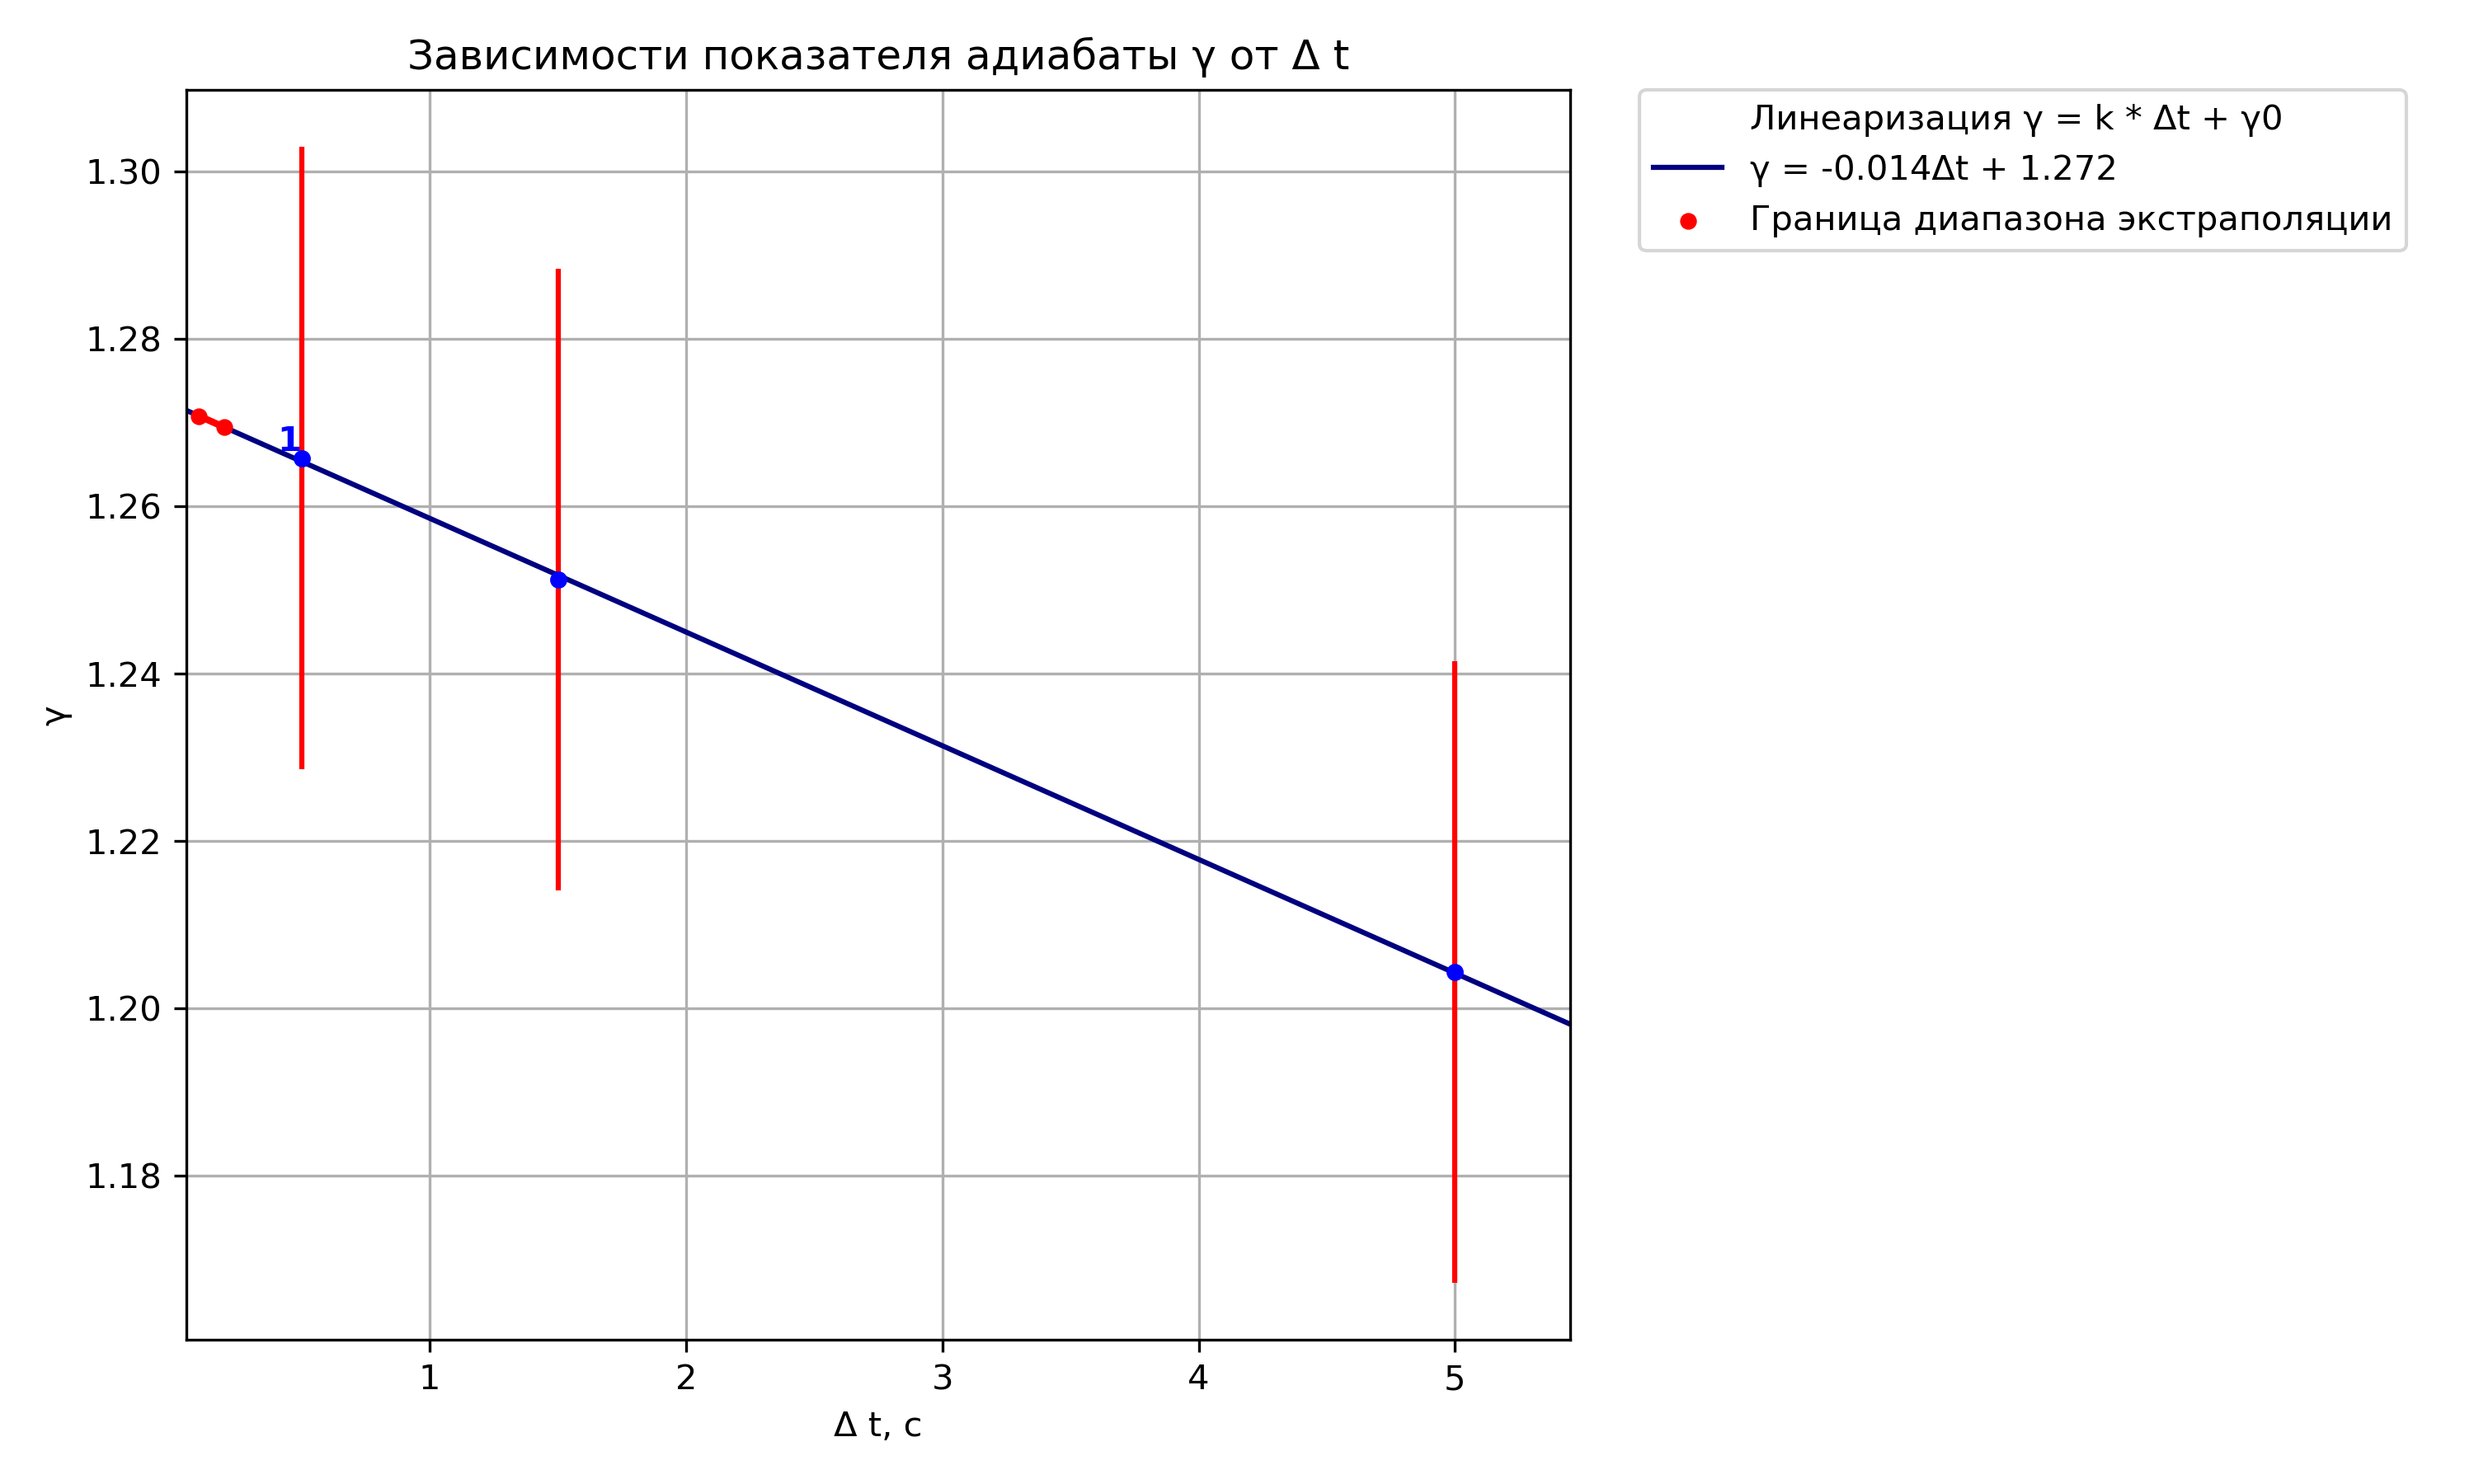
\includegraphics[width=1\textwidth]{graph2.png}}
\caption[]{\label{} График №2 Зависимость показателя адиабаты для углекислого от времени открытия крана $\gamma(\Delta t)$}
\end{figure}

\begin{equation*}
	k = -0,0136 \pm 0,0001
\end{equation*}
\begin{equation*}
	\gamma_0 = 1,2721 \pm 0,0002
\end{equation*}
По полученным параметрам прямой вычисли диапазон показателя адиабаты при $\Delta t$ = 0,1-0,2с.
\begin{equation*}
	\gamma_{CO_2} = 1,2694 - 1,2708
\end{equation*}
\begin{equation*}
	\sigma_{\gamma_{\text{воз}}} = \sqrt{(\Delta t\sigma_k)^2 + \sigma_{\gamma_0}^2} = \sqrt{(1,2 \cdot 10^{-5})^2 + 0,0002^2} = 0,0002
\end{equation*}
\begin{equation*}
	\gamma_{CO_2} = (1,2694\text{\textdiv}1,2708) \pm 0,0002
\end{equation*}

\section{Результаты и обсуждения}
\begin{enumerate}
\item Сравним полученные показатели адиабаты для воздуха и углекислого газа с табличными данными\footnotemark[1]. Для этого рассчитаем молярную теплоемкость воздуха при постоянном давлении с учетом влажности. Давление примем за $P = 101,325$ кПа, температура в комнате $T = 297$ K, влажность $\varphi = 91 \%$. Молярные массы водяного пара и сухого воздуха равны $\mu_{\text{пар}} = 18,0156 \frac{\text{г}}{\text{моль}}$ и $\mu_{\text{воз}} = 28,96 \frac{\text{г}}{\text{моль}}$ соответственно. Плотность воздуха при данной температуре определим с помощью уравнения Менделеева-Клапейрона для идеального газа
\footnotetext[1]{Табличное данные взяты из книги Лабораторный практикум по общей физике Том I Термодинамика и молекулярная физика}
\begin{equation*}
	\rho_{\text{воз}} = \frac{P\mu_{\text{воз}}}{RT} \approx 1,189 \frac{\text{г}}{\text{л}}
\end{equation*}
Плотность насыщенного пара при данной температуре $\rho_{\text{нп}} = 21,8 \frac{\text{г}}{\text{м}^3}$.
Массовые и молярные доли
\begin{equation*}
	\omega_m^{\text{пар}} = \frac{\rho_{\text{пар}}}{\rho_{\text{нп}} + \rho_{\text{воз}}} = \frac{\varphi \cdot \rho_{\text{нп}}}{\rho_{\text{нп}} + \rho_{\text{воз}}} = 0,0164
\end{equation*}
\begin{equation*}
	\omega_m^{\text{воз}} = 0,9836
\end{equation*}
\begin{equation*}
	\omega_\nu^{\text{пар}} = \frac{\frac{\omega_m^{\text{пар}}}{\mu_{\text{пар}}}}{\frac{\omega_m^{\text{пар}}}{\mu_{\text{пар}}} + \frac{\omega_m^{\text{воз}}}{\mu_{\text{воз}}}} = 0,0261
\end{equation*}
\begin{equation*}
	\omega_\nu^{\text{воз}} = 0,9739
\end{equation*}
Молярные теплоемкости водяного пара и сухого воздуха равны $C_p^{\text{пар}} = 34,5$ и $C_p^{\text{воз}} = 29,3$ соответственно. Итоговая теплоемкость влажного воздуха равна
\begin{equation*}
	C_p = \omega_\nu^{\text{воз}}C_p^{\text{воз}} + \omega_\nu^{\text{пар}}C_p^{\text{пар}} = 29,4358
\end{equation*}
Приняв воздух за идеальный газ, используем соотношением Майера и найдем показатель адиабаты влажного воздуха
\begin{equation*}
	\gamma_{\text{воз}}^{\text{табл}} = \frac{C_p}{C_v} = \frac{C_p}{C_p - R} = 1,3868
\end{equation*}
\item Теперь перейдем к сравнению.
\begin{table}[h!]
    \centering
    \begin{tabular}{|c|c|c|c|c|c|c|}
        \hline
        Газ & $\gamma^{\text{эксп}}$ & $\gamma^{\text{табл}}$ & $\sigma_{\gamma}^{\text{эксп}}$ & $\sigma_{\gamma}^{\text{табл}}$ & $\varepsilon_{\gamma}^{\text{эксп}}, \%$ & $\varepsilon_{\gamma}^{\text{табл}}, \%$ \\
        \hline
        Воздух & $1.293$ & $1.3868$ & $0.015$ & $0.0936$ & $1.18$ & $6.75$ \\ \hline
        CO$_2$ & $1.2701$ & $1.3$ & $0.0002$ & $0.0299$ & $0.02$ & $2.30$ \\ \hline
    \end{tabular}
    \caption{Таблица 7. Сравнение экспериментальных и табличных значений $\gamma$ для различных газов}
\end{table}
Значения для $CO_2$ оказались довольно близкими к табличным, точки на графике 2 лежат на прямой с хорошей точностью. Для воздуха значения и график получились менее точными. Это связано с тем, что в первых сериях для воздуха давление $\Delta h_1$ недостаточно для измерений с высокой точностью, нужно было накачивать больше. В то же время для $CO_2$ наоборот для всех серий бралось максимальное допустимое давление, поэтому результаты намного ближе к табличным и погрешность меньше. Также большое расхождение связано с тем, что $\Delta t$ не измерялось с большой точностью, а бралось приблизительное для диапазона. Поэтому графики могут сильно отличаться от ожидаемых. Стоит также напомнить, что итоговая формула (1) получилась с приближением.

\end{enumerate}





\section{Выводы}
По давлению газа определили показатель адиабаты $\gamma$ для воздуха и $CO_2$ для каждого измерения. Построили графики зависимости показателя адиабаты от времени открытия крана $\gamma(\Delta t)$. По экстраполяции определили окончательные показатели адиабаты для газов (см. Таблица 7). Убедились, что экспериментальные значения близки к табличным.

\end{document}